%!TEX root = colt2018.tex


To illustrate our results, we consider one-dimensional synthetic examples ($\X = [0,1] $) for which our assumptions are easily satisfied. 
Indeed, we consider the following set-up that fulfils our assumptions: 
\BIT
\item \asm{asm:separability}, \asm{asm:data-iid} We consider here $X \sim U\left([0,(1-\varepsilon)/2] \cup [(1+\varepsilon)/2,1]  \right)$ and with the notations of Example \ref{ex:independent-noise-on-labels}, we take $S_+ = [0,(1-\varepsilon)/2]$ and $S_- = [(1+\varepsilon)/2,1]$. For $1 \leq i \leq n$,  $x_i$ independently sampled from $\rhox$ we define $y_i = 1 $ if $x_i \in S_+$ and $y_i = -1 $ if $x_i \in S_-$.

\item \asm{asm:kernel-bounded} We take the kernel to be the exponential  kernel $K(x,x') = \exp(-|x-x'|)$ for which the RKHS is a Sobolev space $\H = W^{s,2}$, with $s > d/2$, which is dense in $L_2$~\citet{adams2003sobolev}.

\item \asm{asm:flambda-correct-sign} With this setting we could find a closed form for $g_\lambda$ and checked that it verified \asm{asm:flambda-correct-sign}. Indeed we could solve the optimality equation satisfied by $g_\lambda$ : $$ \forall z \in [0,1], \ \int_{0}^1 K(x,z)g_\lambda(x) d\rho_X(x) + \lambda g_\lambda(z) = \int_{0}^1 K(x,z)g_\rho(x) d\rho_X(x),  $$ the solution being a linear combination of exponentials in each set : $[0,(1-\varepsilon)/2]$, $[(1-\varepsilon)/2,(1+\varepsilon)/2]$ and $[(1+\varepsilon)/2,1]$.
\EIT

\begin{figure}[ht]
    \centering
    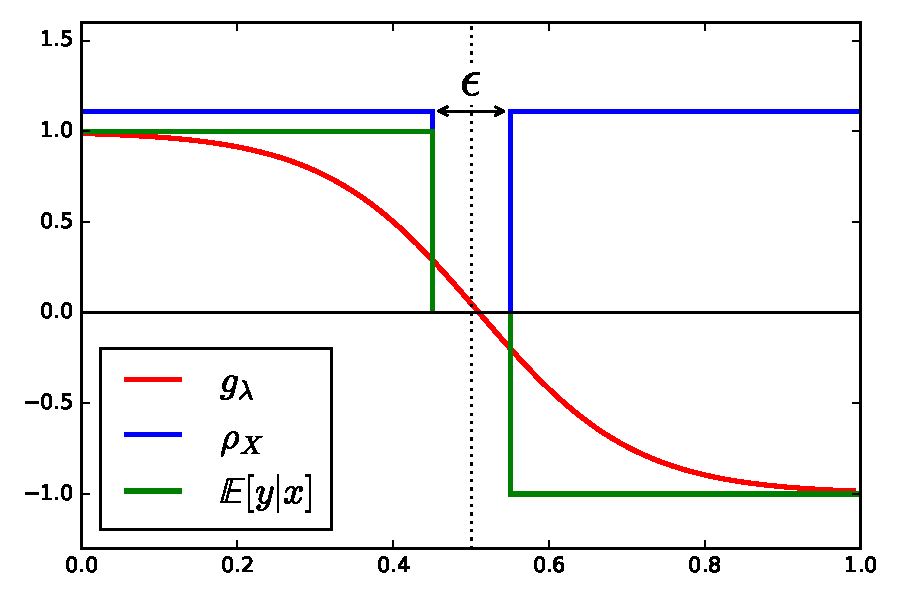
\includegraphics[width=0.45\textwidth]{figures/zbis_densities.pdf}
    \caption{Representing the $\rho_\X$ density (uniform with $\varepsilon$-margin), the best estimator, i.e., $\E (x|y)$ and $g_\lambda$ used for the simulations ($\lambda = 0.01$).}
    \label{fig:densities}
\end{figure}

%
In the case of SGD with decreasing step size, we computed only the test error $\mathbb{E}({\cal R}(g_n)-{\cal R}^*))$. For tail averaged SGD with constant step size, we computed the test error as well as the training error, the test loss (which corresponds to the $L_2$ loss : $\int_0^1 (g_n (x) - g_\lambda(x))^2d\rho(x)$) and the training loss.
%
In all cases we computed the errors of the $n$-th iterate with respect to the calculated $g_\lambda$, taking $g_0 = 0$. For any $n \geqslant 1$,
$$g_n  =  {g}_{n-1} - \gamma_n  \big[ ( {g}_{n-1}(x_n)- y_n)K_{x_n}   + \lambda{g}_{n-1}  \big]. $$

We can use representants to find the recursion on the coefficients. Indeed, if  $g_n = \sum_{i = 1}^n a^n_i K_{x_i},$ then the following recursion for the $(a_i^n)$ reads : 
\begin{eqnarray*}
\text{for } i \leqslant n-1, \ a_i^n &=& (1-\gamma_n \lambda) a_i^{n-1} \\
a_n^n &=& -\gamma_n (\sum_{i = 1}^{n-1} a_i^{n-1} K(x_n,x_i)-y_n).
\end{eqnarray*}
%
From $(a_i^n)$, we can also compute the coefficients of $\bar{g}_n$ and $\bar{g}_n^{\textrm tail}$ that we note $\bar{a}^n_i$ and $\bar{a}^{n,\textrm tail}_i$ respectively: $\bar{a}^n_i = \sum_{k = i}^n \frac{a_i^k}{n+1}$ and $\bar{a}^{n,\textrm tail}_i = \frac{1}{\lfloor n/2 \rfloor}\sum_{k = \lfloor n/2 \rfloor }^n a_i^k.$
%
To show our theoretical results we have decided to present the following figures: 

\BIT
\item For the exponential convergence of the averaged and tail averaged cases, we plotted the error $\log_{10}\mathbb{E}({\cal R}(g_n)-{\cal R}^*))$ as a function of $n$. With this scale and following our results it goes as a line after a certain $n$ (Figures \ref{fig:plots} and \ref{fig:techplots} right).
\item We recover the results of \citet{daft} that show convergence at speed $1/n$ for the loss (Figure \ref{fig:plots} left). We adapted the scale to compare with the error plot.
\item For Figure \ref{fig:techplots} left, we plotted $-\log (- \log (\mathbb{E}({\cal R}(g_n)-{\cal R}^*)) ) $ of the excess error with respect to the $\log$ of $n$ to show a line of slope $-1/2$. It meets our theoretical bound of the form $\exp(-K\sqrt{n})$, 
\EIT

Note that for the plots where we plotted the expected excess errors, i.e., $\mathbb{E}({\cal R}(g_n)-{\cal R}^*)$, we plotted the mean of the errors over 1000 replications until $n = 200$, whereas for the plots where we plotted the losses, i.e., a function of $\|g_n- g_*\|_2$, we plotted the mean of the loss over 100 replications until $n = 2000$.

\begin{figure}[ht]
\footnotesize
\stackunder[1pt]{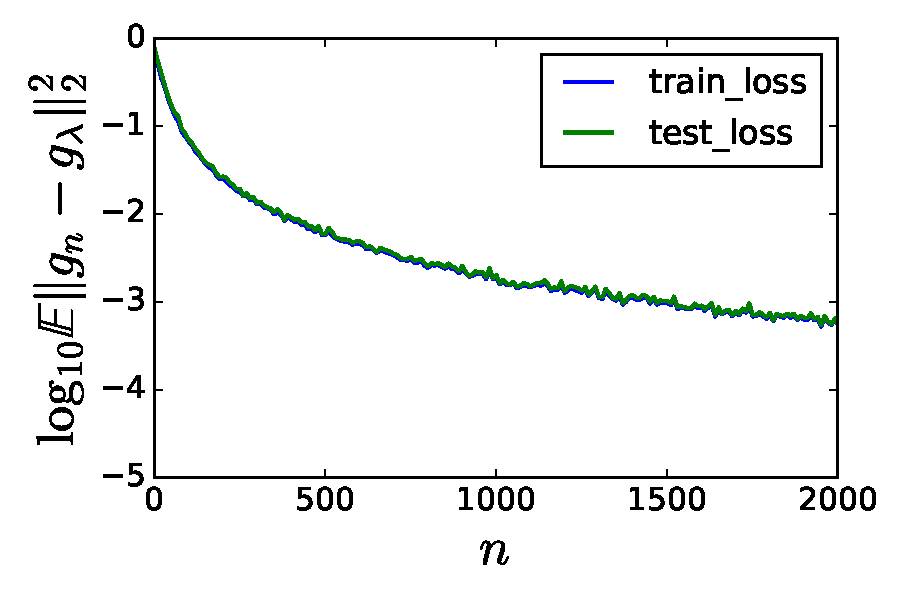
\includegraphics[width=0.48\textwidth]{figures/zbis_a_loss.pdf}}{}%
\hspace{1cm}%
\stackunder[1pt]{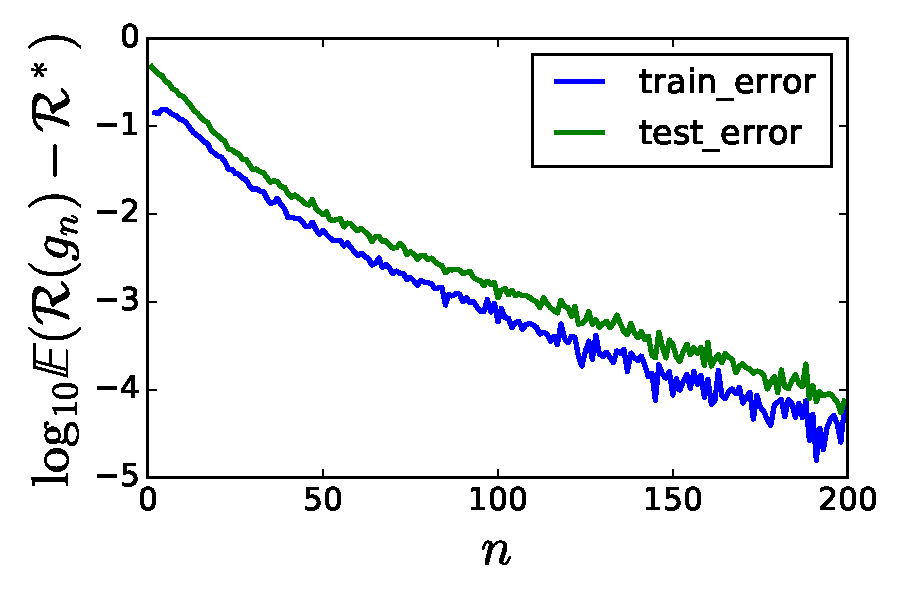
\includegraphics[width=0.48\textwidth]{figures/zbis_a_error.pdf}}{}%
\caption{ \small Showing linear convergence for the $L^{01}$ errors in the case of margin of width $\varepsilon$. {\bfseries Left} figure corresponds to the test and training loss in the averaged case whereas the {\bfseries right} one corresponds to the error in the same setting. Note that the y-axis is the same while the x-axis is different of a factor 10. The fact that the error plot is a line after a certain $n$ matches our theoretical results. We took the following parameters :  $\varepsilon = 0.05$, $\gamma = 0.25$, $\lambda = 0.01$.}
\label{fig:plots}
\end{figure}
%
We can make the following observations:

First remark that between plots of losses and errors (Figure \ref{fig:plots} left and right resp.), there is a factor~10 between the numbers of samples (200 for errors and 2000 for losses) and another factor~10 between errors and losses ($10^{-4}$ for errors and $10^{-3}$ for losses). That underlines well our theoretical result which is the difference between exponential rates of convergence of the excess error and $1/n$ rate of convergence of the loss.

\begin{figure}[ht]
\footnotesize
\stackunder[1pt]{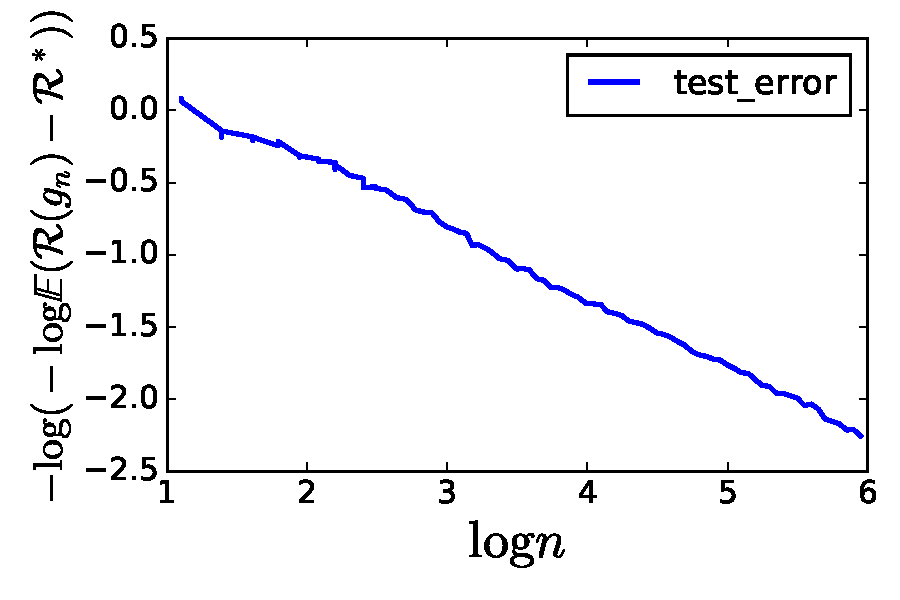
\includegraphics[width=0.48\textwidth]{figures/zbis_error_alpha.pdf}}{}%
\hspace{1cm}%
\stackunder[1pt]{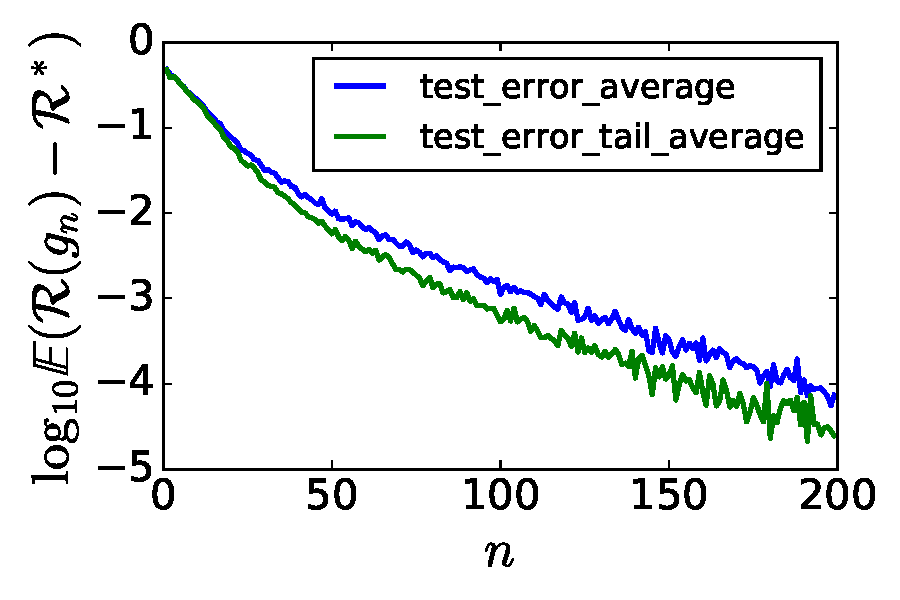
\includegraphics[width=0.48\textwidth]{figures/zbis_error_comparison.pdf}}{}
\caption{ \small {\bfseries Left} plot shows the error in the non-averaged case for $\gamma_n = \gamma / \sqrt{n}$ and {\bfseries right} compares the test error between averaged and tail averaged case. We took the following parameters :  $\varepsilon = 0.05$, $\gamma = 0.25$, $\lambda = 0.01$.}
\label{fig:techplots}
\end{figure}

Moreover, we see that even if the excess error with tail averaging seems a bit faster, we have linear rates too for the convergence of the excess error in the averaged case. Finally, we remark that the error on the train set is always below the one for a unknown test set (of what seems to be close to a factor 2).




